\section{Synthesis objectives and chosen approach\label{section:inductive-objectives-and-approach}}

This section gives a characterization of the synthesis problem and an overview of our solution. Section~\ref{subsection:inductive-synthesis-statement} makes the problem statement precise in terms of the models from Chapter~\ref{chapter:framework}. Section~\ref{subsection:inductive-synthesis-requirements} states additional requirements on the synthesis approach; the problem statement can be strengthened to take each of them into account. Section~\ref{subsection:inductive-synthesis-approach} presents an overview of our inductive-oriented approach in the light of these incremental enhancements.

%%%

\subsection{Problem statement\label{subsection:inductive-synthesis-statement}}

In its simplest form, the problem of synthesizing LTS state machines from MSC scenarios can be stated as follows:

\begin{quotation}
\noindent \underline{Given}~~a consistent MSC collection showing typical examples and counterexamples of system behaviors

\vspace{-0.7cm}
\begin{align*}
Sc = (S^+,S^-)
\end{align*}

\vspace{-0.2cm}
\noindent \underline{Synthesize}~~the system as a composition of agent LTSs

\vspace{-0.7cm}
\begin{align*}
System = (Ag_1 \parallel \ldots \parallel Ag_n)
\end{align*}

\vspace{-0.2cm}
\noindent \underline{Such that}~~$Sc$ and $System$ are consistent.
\end{quotation}

\noindent For recall, the consistency condition covers three criteria (see Section~\ref{subsection:background-scenario-consistency}):

\begin{description}
\item[structural consistency] the state machine and scenario views are \emph{structurally} consistent, that is, they agree on the agent decomposition and their respective interface,

\item[consistent agent view] each timeline of positive scenarios in $S^+$ specifies an existing path in the corresponding agent state machine. The same condition holds for preconditions of negative scenarios in $S^-$.

\item[consistent system view] the system correctly covers all positive scenarios and the preconditions of the negatives ones. It also correctly rejects negative scenarios. The precise conditions from Section~\ref{subsection:background-scenario-consistency} are:
\begin{align*}
\mathcal{L}^+(Sc) & \subseteq \mathcal{L}(System) \\
\mathcal{L}^-(Sc) \cap \mathcal{L}(System) &= \emptyset
\end{align*}
\noindent where $\mathcal{L}^+(Sc)$ and $\mathcal{L}^-(Sc)$ encode the scenario collection in terms of positive and negative event traces, respectively.

\end{description}

%%%

\subsection{Synthesis requirements\label{subsection:inductive-synthesis-requirements}}

The characterization above provides a precise, yet minimal statement in terms of the formal models of Chapter~\ref{chapter:framework}. This statement is completed with a few usability requirements.

\begin{description}
\item[Behavior generalization] -- In most cases, scenarios provide only \emph{examples} of system behaviors and are thus incomplete. Synthesized state machines should cover more behaviors than those described. 

Covering more behaviors is allowed by our formal statement but not enforced. Note that the \emph{consistent system view} condition states an upper bound on behavior generalization, by requiring negative scenarios to be correctly rejected. This upper bound has to be refined if other models are taken into account (see below).

\item[Incremental synthesis] -- The synthesis approach should help incrementally refining a first scenario specification towards richer models.
\begin{itemize}

\item End-users are most likely to be unable to provide rich scenario descriptions in the early phases of system design. This includes state assertions along scenario episodes or flowcharts on such episodes. The synthesis approach should therefore be usable even if only a few scenarios are available.

\item Both positive and negative scenarios should be taken into account. Negative scenarios are not uncommon among the examples provided by stakeholders. One reason is that they naturally illustrate violations of safety goals but are easier to specify than the latter.

\item In an incremental approach to system analysis, richer input scenarios are likely to be \emph{eventually} available. The synthesis should gracefully adapt to work on such richer input in advanced analysis phases. For example, the formal statement might be adapted to take a hMSC as input. 

\end{itemize}

\item[Multi-model synthesis] -- The possibility of having richer input models suggests taking other models into account in the synthesis process, such as fluents or goals. These models should not be \emph{required} as input, but are better \emph{supported} when available. 

In such case, the formal statement must be strengthened. In input, all available models shall be required to be consistent with each other. In output, the synthesized system itself shall be required consistent with all models. Notably, the synthesized system shall not violate known safety goals.

\end{description}

%%%

\subsection{An induction-driven approach\label{subsection:inductive-synthesis-approach}}

Figure~\ref{image:inductive-synthesis-overview} shows the two main steps of our approach for the simple case where a scenario collection is taken as input. 

\begin{figure}[H]\centering
  \scalebox{0.55}{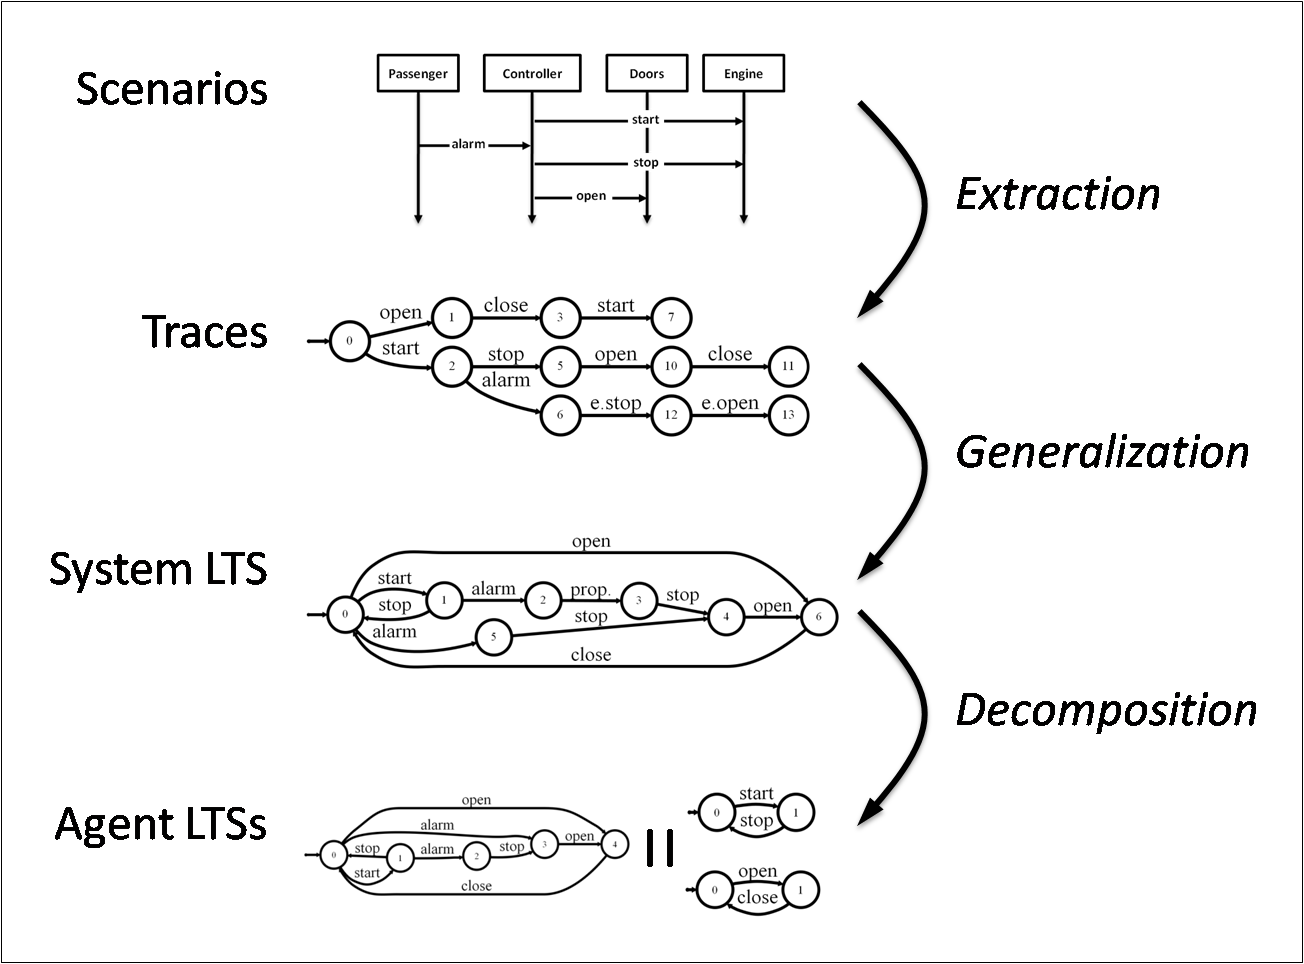
\includegraphics[trim=3mm 3mm 10mm 3mm, clip]{src/4-inductive/images/overview}}
  \caption{Overview of inductive LTS synthesis from MSCs.\label{image:inductive-synthesis-overview}}
\end{figure}

\noindent \textbf{The generalization step} extends grammar induction techniques developed in \cite{Oncina:1992} to synthesize a System LTS covering all positive traces and excluding all negative ones. The generalization strategy is borrowed from the Regular Positive and Negative Inference (RPNI) algorithm and proceeds as follows \cite{Oncina:1992}.

An initial LTS $A_0$ accepting exactly the positive traces is incrementally refined as automata $A_1,\ldots,A_n$ by merging well chosen state pairs. Doing so generalizes accepted behaviors, so that the following relation holds
\begin{align*}
\mathcal{L}(A_n) \subset \ldots \subset \mathcal{L}(A_1) \subset \mathcal{L}(A_0) = \mathcal{L}^+(Sc)
\end{align*}
To avoid over-generalization, this process is performed under the control of the negative traces from $\mathcal{L}^-(Sc)$. Every intermediate solution $A_i$ respects the \emph{consistent system view} condition; the latter therefore provides a useful algorithm invariant:
\begin{align*}
\mathcal{L}^+(Sc) & \subseteq \mathcal{L}(A_i) \\
\mathcal{L}^-(Sc) \cap \mathcal{L}(A_i) &= \emptyset
\end{align*}

\noindent \textbf{The decomposition step} computes a LTS for each agent by projecting the System LTS onto their respective alphabet. For an agent $Ag$ the projection of the System LTS $S$ is given by:
\begin{align}
(S \setminus \Sigma_{Ag}^c)^\Delta
\end{align}
\noindent where $\Sigma_{Ag}^c$ denotes the set of all system events but those of $Ag$'s interface.

The above formula makes use of the hiding, determinization and minimization operators on LTS discussed in Section~\ref{section:background-state-machines}.

\subsubsection*{A word about correctness}

The decomposition step guarantees that the \emph{structural consistency} and \emph{consistent agent view} conditions hold. It is a straightforward application of the material given in Chapter~\ref{chapter:framework}. 

The generalization invariant guarantees that the \emph{consistent system view} condition holds for the System LTS. Strictly speaking, the approach is correct only if this condition holds for the system re-composition $\system$. This might not be the case in presence of negative implied scenarios. This issue is further examined in Section~\ref{section:inductive-discussion}.

\subsubsection*{Integration of additional requirements}

The generalization step is driven by RPNI; this provides a first milestone towards an inductive LTS synthesis approach that meets our requirements. Indeed, it generalizes scenario behaviors without requiring additional state or flowchart information. However, such approach does not provide much support for incremental system analysis; multi-model consistency is not guaranteed either. Section \ref{section:inductive-background} covers this first milestone through background on grammar induction and RPNI.

Section~\ref{section:lts-induction-from-mscs} introduces the Query-driven State Merging (QSM) algorithm that extends RPNI with an interactive feature. The latter supports the elicitation of additional, ``interesting'' scenarios that are not originally provided by the end-user. The original collection of scenarios is completed by asking the user scenario queries that are generated during synthesis. A \emph{scenario query} consists of showing the user a specific scenario and asking her to classify it as positive or negative. This guides the generalization process towards more accurate state machines while incrementally enriching an initial scenario collection.

The multi-view synthesis requirement is tackled in Section~\ref{section:inductive-mutliview-consistency}. QSM is extended so as to allow the injection of additional information that constrain the induction and prune the inductive search space. Additional information may include global definitions of fluents; declarative properties of the domain; behavior models of external components; and goals that the system is expected to satisfy. Doing so guarantees the consistency of synthesized state machines with all other models.

Managing the consistency of a large scenario collection is challenging; hMSCs partly address this through a structured form of scenarios that allows reuse. Section~\ref{section:inductive-from-hMSC} shows how hMSCs can replace scenario collections as input of the generalization process. In this setting, negative scenarios and other models can still be used to constraint induction so as to achieve multi-view consistency. At the time of writing, however, the interactive feature of QSM is still a work in progress.

Taking hMSCs as input implies both a theoretical and practical shift of perspective. It leads us considering the generalization of state machines under the control of safety goals as a synthesis technique that naturally succeeds the generalization of positive scenario behaviors under the control of negative ones. Among others, this perspective is further discussed in Section~\ref{section:inductive-discussion}.
